\documentclass[aspectratio=169, table, 12pt]{beamer}

\usepackage{colortbl}
\usepackage{xcolor}
\usepackage{listings}
\usepackage{tabularx}
\usepackage{tikz}
\usetikzlibrary{arrows.meta, positioning, calc, fit, shapes.geometric}

\makeatletter
\def\input@path{{../theme/}}
\makeatother
\graphicspath{{../theme/}{../../figures/}}
\usetheme{Pradita}

\definecolor{praditagreen}{RGB}{37, 113, 71}

% Tema membuat garis tabel berwarna putih. Dikembalikan agar tabel terbaca.
\arrayrulecolor{black}
\setlength{\arrayrulewidth}{0.5pt}

% Kolom X rata kiri, dipakai pada tabel dengan kolom X yang sempit, agar
% spasi antarkata tidak meregang.
\newcolumntype{Y}{>{\raggedright\arraybackslash}X}

\lstdefinelanguage{bash}{
  keywords={},
  basicstyle=\ttfamily\scriptsize,
  ndkeywords={cd, curl, python3},
  ndkeywordstyle=\color{purple}\bfseries,
  sensitive=true,
  commentstyle=\color{gray},
  numbers=none,
  breaklines=true,
  frame=lines,
  backgroundcolor=\color{lightgray!10},
  tabsize=2,
  comment=[l]{\#},
  showstringspaces=false
}

\lstdefinelanguage{yaml}{
  keywords={},
  basicstyle=\ttfamily\scriptsize,
  commentstyle=\color{gray},
  stringstyle=\color{red},
  numbers=none,
  breaklines=true,
  frame=lines,
  backgroundcolor=\color{lightgray!10},
  tabsize=2,
  comment=[l]{\#},
  morestring=[b]",
  showstringspaces=false
}

% Gaya Python disamakan dengan naskah bab, tanpa nomor baris.
\lstdefinestyle{PythonStyle}{
  language=Python,
  basicstyle=\ttfamily\scriptsize,
  morekeywords={with, as, yield, async, await, match, case},
  keywordstyle=\color{blue}\bfseries,
  emph={socket},
  emphstyle=\color{purple}\bfseries,
  commentstyle=\color{gray}\itshape,
  stringstyle=\color{red},
  numbers=none,
  breaklines=true,
  frame=lines,
  backgroundcolor=\color{lightgray!10},
  tabsize=2,
  showstringspaces=false
}

\title{\Huge Overview Mata Kuliah\\ \vspace{10pt} dan Alur Rekayasa}
\subtitle{IF140303 - Pengembangan Aplikasi Web}
\author{\textbf{Alfa Yohannis}}

\begin{document}

\frame{\titlepage}

\begin{frame}[fragile]
  \frametitle{Isi Pertemuan}
  \vspace{14pt}
  \begin{columns}[t]
    \column{0.5\textwidth}
    {\small\tableofcontents[sections={1-6}]}

    \column{0.5\textwidth}
    {\small\tableofcontents[sections={7-12}]}
  \end{columns}
\end{frame}

\begin{frame}{\hfill}
  \centering
  \Huge{\textbf{Aplikasinya sudah berjalan.\\Seberapa baik?}}
\end{frame}

\section{Tujuan dan Posisi Mata Kuliah}

\begin{frame}{\hfill}
  \centering
  \Huge{\textbf{Tujuan dan Posisi\\Mata Kuliah}}
\end{frame}

\begin{frame}{{\Large Tujuan Pembelajaran}}
  \vspace{10pt}
  \begin{itemize}
    \item Menjelaskan beda mata kuliah ini dengan pemrograman web pengantar,
          beserta peta empat belas pertemuannya.
    \item Memeriksa kesiapan lingkungan kerja untuk keempat belas bab dengan
          satu \textit{smoke test}, lalu menjelaskan tiap pemeriksaan yang
          gagal.
    \item Merancang alur kerja tim: monorepo, cabang berumur pendek,
          \textit{code review}, dan Continuous Integration (CI).
  \end{itemize}
\end{frame}

\begin{frame}{{\Large Pertanyaan yang Berubah}}
  \vspace{6pt}
  \centering
  {\footnotesize
  \begin{tabularx}{\textwidth}{lYY}
    \hline
    \textbf{Aspek} & \textbf{Pengantar} & \textbf{Mata kuliah ini} \\
    \hline
    pertanyaan utama & apakah fiturnya berjalan & seberapa baik berjalan, dan buktinya \\
    \hline
    bukti & demo di depan kelas & angka hasil pengukuran, misalnya p95 \\
    \hline
    lingkungan & satu laptop, satu proses & \textit{container}, beberapa layanan, beban \\
    \hline
    kegagalan & dihindari & disengaja, diukur, lalu diredam \\
    \hline
    mutu kode & lulus bila berjalan & diuji otomatis dan dijaga CI \\
    \hline
  \end{tabularx}}

  \vspace{6pt}
  {\small Seperti beda menyetir mobil sendiri dengan mengemudikan bus kampus
  terjadwal: keduanya sampai tujuan, tetapi bus dinilai dari catatan
  perjalanannya.}
\end{frame}

\begin{frame}{{\Large Jenis Jawaban yang Dicari}}
  \vspace{12pt}
  \begin{itemize}
    \item Bab 13: sepuluh peristiwa yang sama tiba dalam 199,8 ms lewat
          \textit{polling}, dan dalam 1,8 ms lewat sambungan yang mendorong.
    \item Bab 14: satu ke delapan replika menaikkan \textit{throughput} dari
          106,8 menjadi 198,0 permintaan per detik, lalu berhenti karena basis
          datanya penuh.
    \item p50 tidak dilampaui separuh permintaan, p95 tidak dilampaui 95 dari
          100. Yang kedua lebih jujur.
  \end{itemize}
\end{frame}

\section{Peta Empat Belas Pertemuan}

\begin{frame}{\hfill}
  \centering
  \Huge{\textbf{Peta Empat Belas\\Pertemuan}}
\end{frame}

\begin{frame}{{\Large Empat Bagian}}
  \vspace{10pt}
  \centering
  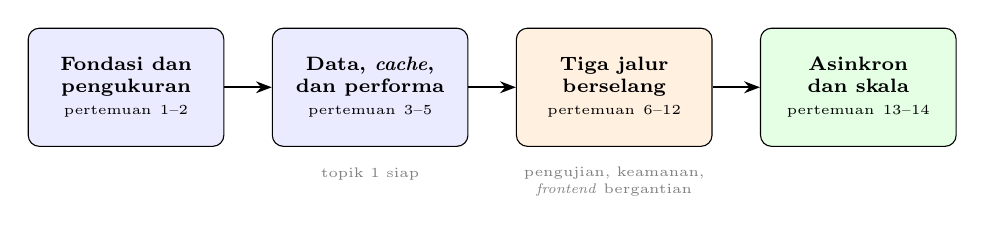
\begin{tikzpicture}[
    font=\scriptsize,
    kotak/.style={draw, rounded corners, minimum height=1.5cm,
                  text width=2.25cm, align=center, font=\scriptsize\bfseries},
    panah/.style={-{Stealth[length=2mm]}, thick}
  ]
    \node[kotak, fill=blue!8] (bagian1) at (0,0) {Fondasi dan pengukuran\\{\tiny\mdseries pertemuan 1--2}};
    \node[kotak, fill=blue!8] (bagian2) at (3.1,0) {Data, \textit{cache}, dan performa\\{\tiny\mdseries pertemuan 3--5}};
    \node[kotak, fill=orange!12] (bagian3) at (6.2,0) {Tiga jalur berselang\\{\tiny\mdseries pertemuan 6--12}};
    \node[kotak, fill=green!10] (bagian4) at (9.3,0) {Asinkron dan skala\\{\tiny\mdseries pertemuan 13--14}};

    \draw[panah] (bagian1) -- (bagian2);
    \draw[panah] (bagian2) -- (bagian3);
    \draw[panah] (bagian3) -- (bagian4);
    \node[font=\tiny, gray] at (3.1,-1.1) {topik 1 siap};
    \node[font=\tiny, gray, align=center] at (6.2,-1.2) {pengujian, keamanan,\\\textit{frontend} bergantian};
  \end{tikzpicture}

  \vspace{8pt}
  {\small Satu aplikasi dipakai sepanjang semester: toko buku kampus dengan
  50.000 buku, 20.000 pelanggan, dan 200.000 pesanan mulai Bab 3.}
\end{frame}

\begin{frame}{{\Large Enam Topik Penelitian}}
  \vspace{6pt}
  \centering
  {\footnotesize
  \begin{tabularx}{\textwidth}{lYll}
    \hline
    \textbf{Topik} & \textbf{Masalah yang diteliti} & \textbf{Pertemuan} & \textbf{Siap sesudah} \\
    \hline
    T1 & invalidasi \textit{cache} hibrida & 3, 4, 5 & pertemuan 5 \\
    \hline
    T2 & pencabutan token di \textit{gateway} & 7, 10, 12 & pertemuan 12 \\
    \hline
    T3 & transport \textit{real-time} adaptif & 5, 13 & pertemuan 13 \\
    \hline
    T4 & \textit{semantic cache} untuk Large Language Model (LLM) & 4, 5, 14 & pertemuan 14 \\
    \hline
    T5 & hidrasi selektif & 5, 8, 11 & pertemuan 11 \\
    \hline
    T6 & \textit{gate} kinerja di CI & 3, 6, 9 & pertemuan 9 \\
    \hline
  \end{tabularx}}
\end{frame}

\section{Tech Stack}

\begin{frame}{\hfill}
  \centering
  \Huge{\textbf{Tech Stack}}
\end{frame}

\begin{frame}{{\Large Perkakas dan Alasannya}}
  \vspace{4pt}
  \centering
  {\footnotesize
  \begin{tabularx}{\textwidth}{llY}
    \hline
    \textbf{Kebutuhan} & \textbf{Pilihan} & \textbf{Alasan} \\
    \hline
    server dan alat ukur & Python 3 & kode terbaca, pustaka standarnya cukup untuk HTTP \\
    \hline
    kode di browser & JavaScript, TypeScript & memang berjalan di browser \\
    \hline
    basis data & PostgreSQL 16 & rencana \textit{query} terlihat jelas \\
    \hline
    \textit{cache} & Redis 7 & \textit{cache} di luar proses \\
    \hline
    lingkungan & Docker Compose & basis data yang sama di tiap laptop \\
    \hline
    pengukuran browser & Chrome, Playwright & membuka halaman tanpa jendela \\
    \hline
    versi & Git, satu monorepo & naskah, slide, dan kode berubah bersama \\
    \hline
  \end{tabularx}}

  \vspace{4pt}
  {\small Yang terukur harus mekanismenya, bukan \textit{framework}-nya.}
\end{frame}

\section{Smoke Test Lingkungan}

\begin{frame}{\hfill}
  \centering
  \Huge{\textbf{Smoke Test Lingkungan}}
\end{frame}

\begin{frame}[fragile]{{\Large Memeriksa Port Tanpa Mengirim Data}}
  \vspace{2pt}
\begin{lstlisting}[style=PythonStyle]
def port_terpakai(port):
  with socket.socket(socket.AF_INET, socket.SOCK_STREAM) as soket:
    soket.setsockopt(socket.SOL_SOCKET, socket.SO_REUSEADDR, 1)
    try:
      soket.bind(("", port))
    except OSError:
      return True
  return False
\end{lstlisting}
  \vspace{2pt}
  {\small Seperti daftar periksa di laboratorium: alat yang rusak ketahuan
  dalam lima menit, bukan di tengah percobaan yang bahannya telanjur
  dicampur.}
\end{frame}

\begin{frame}{{\Large Hasilnya di Laptop Penulis}}
  \vspace{4pt}
  \centering
  {\footnotesize
  \begin{tabularx}{\textwidth}{YlY}
    \hline
    \textbf{Pemeriksaan} & \textbf{Hasil} & \textbf{Keterangan} \\
    \hline
    Python, Node.js, npm, Git & lolos & 3.15.2, v22.23.4, 10.9.9, 2.43.0 \\
    \hline
    Docker dan Docker Compose & lolos & server 29.9.3, Compose 5.7.0 \\
    \hline
    Chrome atau Chromium & lolos & 157.0.8103.38 \\
    \hline
    psycopg di \texttt{sources/.venv} & lolos & 3.3.5 \\
    \hline
    port bab 1 sampai 14 & gagal & 3 dari 37 terpakai: 5433, 8000, 8080 \\
    \hline
  \end{tabularx}}

  \vspace{4pt}
  {\small Ketiga port dipakai proyek lain, padahal milik Bab 3, Bab 4, dan
  Bab 11. Tanpa pemeriksaan ini, kegagalannya baru muncul berminggu-minggu
  kemudian.}
\end{frame}

\section{Monorepo dan Branching}

\begin{frame}{\hfill}
  \centering
  \Huge{\textbf{Monorepo dan Branching}}
\end{frame}

\begin{frame}{{\Large Satu Repositori untuk Seluruh Bagian}}
  \vspace{10pt}
  \centering
  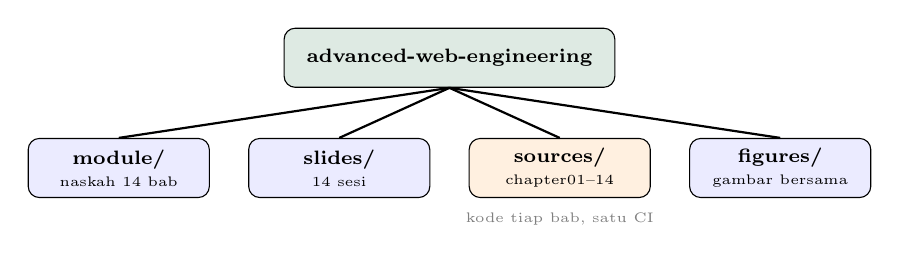
\begin{tikzpicture}[
    font=\scriptsize,
    kotak/.style={draw, rounded corners, minimum height=0.75cm,
                  minimum width=2.3cm, align=center, font=\scriptsize\bfseries},
    panah/.style={-{Stealth[length=2mm]}, thick}
  ]
    \node[kotak, fill=praditagreen!15, minimum width=4.2cm] (akar) at (4.2,1.4) {advanced-web-engineering};
    \node[kotak, fill=blue!8] (module) at (0,0) {module/\\{\tiny\mdseries naskah 14 bab}};
    \node[kotak, fill=blue!8] (slides) at (2.8,0) {slides/\\{\tiny\mdseries 14 sesi}};
    \node[kotak, fill=orange!12] (sources) at (5.6,0) {sources/\\{\tiny\mdseries chapter01--14}};
    \node[kotak, fill=blue!8] (figures) at (8.4,0) {figures/\\{\tiny\mdseries gambar bersama}};
    \foreach \anak in {module, slides, sources, figures} {
      \draw[thick] (akar.south) -- (\anak.north);
    }
    \node[font=\tiny, gray] at (5.6,-0.65) {kode tiap bab, satu CI};
  \end{tikzpicture}

  \vspace{8pt}
  {\small Seperti satu lemari arsip fakultas dengan laci tiap program studi:
  aturan baru diperbarui sekaligus, dan tidak ada \textit{copy} lama yang
  tertinggal di rumah seseorang.}
\end{frame}

\begin{frame}{{\Large Umur Cabang dan Konflik, Diukur}}
  \vspace{6pt}
  \centering
  {\footnotesize
  \begin{tabularx}{\textwidth}{Yllll}
    \hline
    \textbf{Umur cabang} & \textbf{Diubah A} & \textbf{Diubah B} & \textbf{Diubah keduanya} & \textbf{Blok konflik} \\
    \hline
    1 hari & 3 & 3 & 0 & 0 \\
    \hline
    3 hari & 9 & 9 & 0 & 0 \\
    \hline
    7 hari & 20 & 19 & 1 & 3 \\
    \hline
    14 hari & 40 & 39 & 2 & 11 \\
    \hline
  \end{tabularx}}

  \vspace{6pt}
  {\small Dua baris diubah keduanya, tetapi blok konfliknya sebelas: Git juga
  menolak dua perubahan pada baris yang berdampingan. Konflik tumbuh lebih
  cepat daripada umur cabangnya.}
\end{frame}

\section{Code Review}

\begin{frame}{\hfill}
  \centering
  \Huge{\textbf{Code Review}}
\end{frame}

\begin{frame}{{\Large Aturan Sepanjang Semester}}
  \vspace{6pt}
  \centering
  {\footnotesize
  \begin{tabularx}{\textwidth}{YY}
    \hline
    \textbf{Aturan} & \textbf{Alasan} \\
    \hline
    satu perubahan, satu tujuan, sekitar 100 baris & 1.000 baris umumnya terlalu besar untuk dibaca teliti \\
    \hline
    CI hijau sebelum diminta dibaca & pembaca tidak membuang waktu pada kesalahan mesin \\
    \hline
    minimal satu pembaca selain penulis & penulis paling sulit melihat kesalahannya sendiri \\
    \hline
    komentar tentang kode, bukan tentang orang & penulisnya tetap mau meminta \textit{review} \\
    \hline
  \end{tabularx}}
\end{frame}

\section{Continuous Integration}

\begin{frame}{\hfill}
  \centering
  \Huge{\textbf{Continuous Integration}}
\end{frame}

\begin{frame}{{\Large Langkah Termurah Lebih Dahulu}}
  \vspace{10pt}
  \centering
  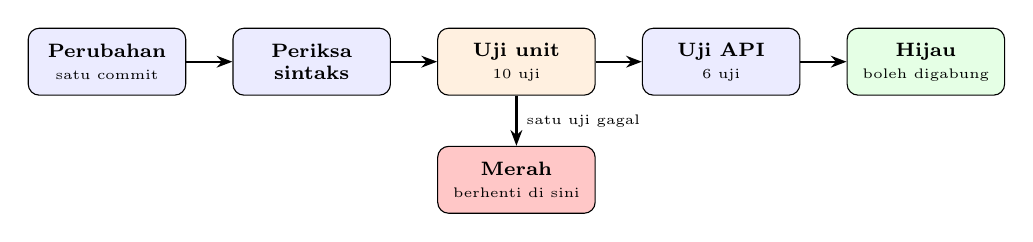
\begin{tikzpicture}[
    font=\scriptsize,
    kotak/.style={draw, rounded corners, minimum height=0.85cm,
                  minimum width=2.0cm, align=center, font=\scriptsize\bfseries},
    panah/.style={-{Stealth[length=2mm]}, thick}
  ]
    \node[kotak, fill=blue!8] (commit) at (0,0) {Perubahan\\{\tiny\mdseries satu commit}};
    \node[kotak, fill=blue!8] (sintaks) at (2.6,0) {Periksa\\sintaks};
    \node[kotak, fill=orange!12] (unit) at (5.2,0) {Uji unit\\{\tiny\mdseries 10 uji}};
    \node[kotak, fill=blue!8] (api) at (7.8,0) {Uji API\\{\tiny\mdseries 6 uji}};
    \node[kotak, fill=green!10] (hijau) at (10.4,0) {Hijau\\{\tiny\mdseries boleh digabung}};
    \node[kotak, fill=red!22] (merah) at (5.2,-1.5) {Merah\\{\tiny\mdseries berhenti di sini}};

    \draw[panah] (commit) -- (sintaks);
    \draw[panah] (sintaks) -- (unit);
    \draw[panah] (unit) -- (api);
    \draw[panah] (api) -- (hijau);
    \draw[panah] (unit) -- node[font=\tiny, right] {satu uji gagal} (merah);
  \end{tikzpicture}

  \vspace{8pt}
  {\small Seperti pemeriksa naskah di percetakan: salah ketik ditolak sebelum
  masuk mesin cetak, bukan sesudah 500 eksemplar tercetak.}
\end{frame}

\begin{frame}[fragile]{{\Large Workflow CI Bab Ini}}
  \vspace{2pt}
\begin{lstlisting}[language=yaml, basicstyle=\ttfamily\tiny]
on:
  push:
    branches: [main]
    paths: ["sources/chapter01/**"]
  pull_request:
    paths: ["sources/chapter01/**"]

jobs:
  periksa:
    runs-on: ubuntu-latest
    steps:
      - uses: actions/checkout@v4
      - uses: actions/setup-python@v5
        with:
          python-version: "3.12"

      - name: Sintaks, uji unit, dan uji API
        run: python3 sources/chapter01/ci-lokal.py
\end{lstlisting}
  \vspace{2pt}
  {\small Filter \texttt{paths} membuat \textit{pipeline} ini hanya berjalan
  ketika bagian monorepo miliknya berubah.}
\end{frame}

\begin{frame}{{\Large Utuh Lawan Dirusak, Diukur}}
  \vspace{6pt}
  \centering
  {\footnotesize
  \begin{tabularx}{\textwidth}{Yllll}
    \hline
    \textbf{Langkah} & \textbf{Utuh} & \textbf{Detik} & \textbf{Dirusak} & \textbf{Detik} \\
    \hline
    periksa sintaks & lolos & 0,04 & lolos & 0,04 \\
    \hline
    uji unit \textit{service} & lolos & 0,06 & gagal & 0,07 \\
    \hline
    uji API lewat HTTP & lolos & 0,10 & tidak dijalankan & - \\
    \hline
    \textbf{hasil} & \textbf{hijau} & & \textbf{merah} & \\
    \hline
  \end{tabularx}}

  \vspace{6pt}
  {\small Buku seharga nol tertahan dalam 0,07 detik dengan nama uji
  \texttt{test\_harga\_nol\_ditolak}, sebelum ada orang yang membacanya.}
\end{frame}

\section{Route, Service, Repository}

\begin{frame}{\hfill}
  \centering
  \Huge{\textbf{Route, Service,\\Repository}}
\end{frame}

\begin{frame}{{\Large Tiga Lapisan API}}
  \vspace{10pt}
  \centering
  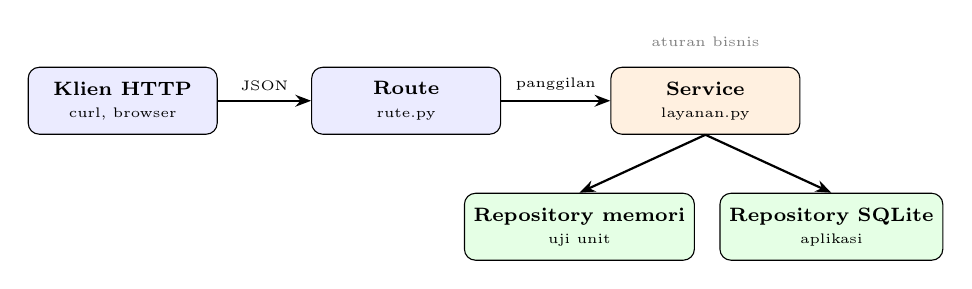
\begin{tikzpicture}[
    font=\scriptsize,
    kotak/.style={draw, rounded corners, minimum height=0.85cm,
                  minimum width=2.4cm, align=center, font=\scriptsize\bfseries},
    panah/.style={-{Stealth[length=2mm]}, thick}
  ]
    \node[kotak, fill=blue!8] (http) at (0,0) {Klien HTTP\\{\tiny\mdseries curl, browser}};
    \node[kotak, fill=blue!8] (rute) at (3.6,0) {Route\\{\tiny\mdseries rute.py}};
    \node[kotak, fill=orange!12] (layanan) at (7.4,0) {Service\\{\tiny\mdseries layanan.py}};
    \node[kotak, fill=green!10] (memori) at (5.8,-1.6) {Repository memori\\{\tiny\mdseries uji unit}};
    \node[kotak, fill=green!10] (sqlite) at (9.0,-1.6) {Repository SQLite\\{\tiny\mdseries aplikasi}};

    \draw[panah] (http) -- node[font=\tiny, above] {JSON} (rute);
    \draw[panah] (rute) -- node[font=\tiny, above] {panggilan} (layanan);
    \draw[panah] (layanan.south) -- (memori.north);
    \draw[panah] (layanan.south) -- (sqlite.north);
    \node[font=\tiny, gray] at (7.4,0.75) {aturan bisnis};
  \end{tikzpicture}

  \vspace{8pt}
  {\small Seperti loket uang kuliah: petugas loket menerima formulir, bagian
  keuangan menghitung denda, arsip menyimpan berkas. Arsip yang pindah ruangan
  tidak mengubah kerja loket.}
\end{frame}

\begin{frame}[fragile]{{\Large Aturan Bisnis di Service}}
  \vspace{2pt}
\begin{lstlisting}[style=PythonStyle]
    if not bilangan_bulat(harga) or harga < HARGA_MINIMUM_RUPIAH:
      raise KesalahanValidasi("harga harus bilangan bulat positif")
    if not bilangan_bulat(stok) or stok < STOK_MINIMUM:
      raise KesalahanValidasi("stok harus bilangan bulat, tidak negatif")
    return self.repositori.simpan(judul, harga, stok)
\end{lstlisting}
  \vspace{4pt}
  {\small
  \begin{tabularx}{\textwidth}{Ylll}
    \hline
    \textbf{Lapisan yang diuji} & \textbf{Uji} & \textbf{Detik} & \textbf{Butuh} \\
    \hline
    \textit{service}, \textit{repository} memori & 10 & di bawah 0,001 & tidak ada \\
    \hline
    API lewat HTTP, SQLite & 6 & 0,016 & server dan basis data \\
    \hline
  \end{tabularx}}
\end{frame}

\section{Persiapan Latihan}

\begin{frame}{\hfill}
  \centering
  \Huge{\textbf{Persiapan Latihan}}
\end{frame}

\begin{frame}[fragile]{{\Large Python 3 dan Git Saja}}
  \vspace{2pt}
\begin{lstlisting}[language=bash]
cd sources/chapter01
python3 -m venv ../.venv
../.venv/bin/pip install "psycopg[binary,pool]"
# Dua perintah di atas cukup sekali, bila sources/.venv belum ada.
python3 periksa-lingkungan.py
\end{lstlisting}
  \vspace{2pt}
  {\small Seluruh skrip hanya menyentuh komputer sendiri. Pemeriksaan port
  memesan tiap port sebentar lalu melepasnya, dan percobaan Git berjalan di
  direktori sementara.}
\end{frame}

\section{Latihan 1 dan 2}

\begin{frame}{\hfill}
  \centering
  \Huge{\textbf{Latihan 1 dan 2:\\Lingkungan dan Cabang}}
\end{frame}

\begin{frame}[fragile]{{\Large Smoke Test dan Umur Cabang}}
  \vspace{2pt}
\begin{lstlisting}[language=bash]
python3 periksa-lingkungan.py | tail -5
# Keluarannya:
#     port 5433 milik Bab 3 sedang dipakai proses lain
#     port 8000 milik Bab 4 sedang dipakai proses lain
#     port 8080 milik Bab 11 sedang dipakai proses lain
#
#   Hasil: merah, 1 pemeriksaan gagal

python3 simulasi-cabang.py | tail -2
# Keluarannya:
#        7 hari        20        19                1             3
#       14 hari        40        39                2            11
\end{lstlisting}
  \vspace{2pt}
  {\small Lalu ubah \texttt{BARIS\_PER\_HARI} menjadi 6. Blok konfliknya
  menjadi 0, 2, 10, dan 21.}
\end{frame}

\section{Latihan 3}

\begin{frame}{\hfill}
  \centering
  \Huge{\textbf{Latihan 3:\\API dan CI yang Hijau}}
\end{frame}

\begin{frame}[fragile]{{\Large CI Lokal dan Tiga Permintaan}}
  \vspace{2pt}
\begin{lstlisting}[language=bash]
python3 ci-lokal.py | tail -1
# Keluarannya:
#   Hasil: hijau, seluruh langkah lolos

python3 aplikasi.py &
# Tiga permintaan curl, status HTTP di ujung tiap baris:
# {"nomor": 1, "judul": "Basis Data Terapan", "harga": 85000, "stok": 4} 201
# {"pesan": "harga harus bilangan bulat positif"} 400
# {"pesan": "buku nomor 9 tidak ada"} 404
\end{lstlisting}
  \vspace{2pt}
  {\small Dengan aturan harga yang dirusak, permintaan kedua dijawab 201: buku
  gratis benar-benar masuk katalog. CI menahannya lebih dahulu.}
\end{frame}

\section{Ringkasan}

\begin{frame}{\hfill}
  \centering
  \Huge{\textbf{Ringkasan}}
\end{frame}

\begin{frame}{{\Large Ringkasan}}
  \vspace{8pt}
  \begin{itemize}
    \item Mata kuliah ini menilai sifat yang tidak terlihat di layar, dan
          jawabannya selalu angka yang diukur sendiri.
    \item \textit{Smoke test} menemukan tiga dari 37 port sudah terpakai
          pada pertemuan pertama, bukan di tengah praktikum.
    \item Cabang satu atau tiga hari bebas konflik, cabang dua minggu
          menimbulkan 11 blok konflik.
    \item CI hijau dalam 0,20 detik, dan kode yang dirusak tertahan di uji
          unit dalam 0,07 detik.
    \item Kebiasaan kerja ditetapkan sejak awal dan dijaga mesin.
  \end{itemize}
\end{frame}

\end{document}
